\chapter{Multi channel APR system details}\label{ap:MultiAPRsystem}

\ifpdf
    \graphicspath{{Appendices/AppendixMultiAPRsystem/Photos/}{Appendices/AppendixMultiAPRsystem/Figs/}}
\else
\fi

As seen in Figure~\ref{fig:MultiAPRsystem.pdf}, on page~\pageref{fig:MultiAPRsystem.pdf}, and Figure~\ref{fig:multiAPRsystemwhole}(a) the multichannel APR system was constructed of a block of medium-density fibreboard wood \todo{Insert measurements}, with 6 1cm diameter 2 cm deep holes drilled into it from the back. On the front of the surface a grid was marked out and 9 points were marked out. These 9 spots can be seen as squares drawn in pencil on Figure~\ref{fig:multiAPRsystemwhole}(b).


\begin{figure}
\centering
\begin{subfigure}{.5\textwidth}
  \centering
  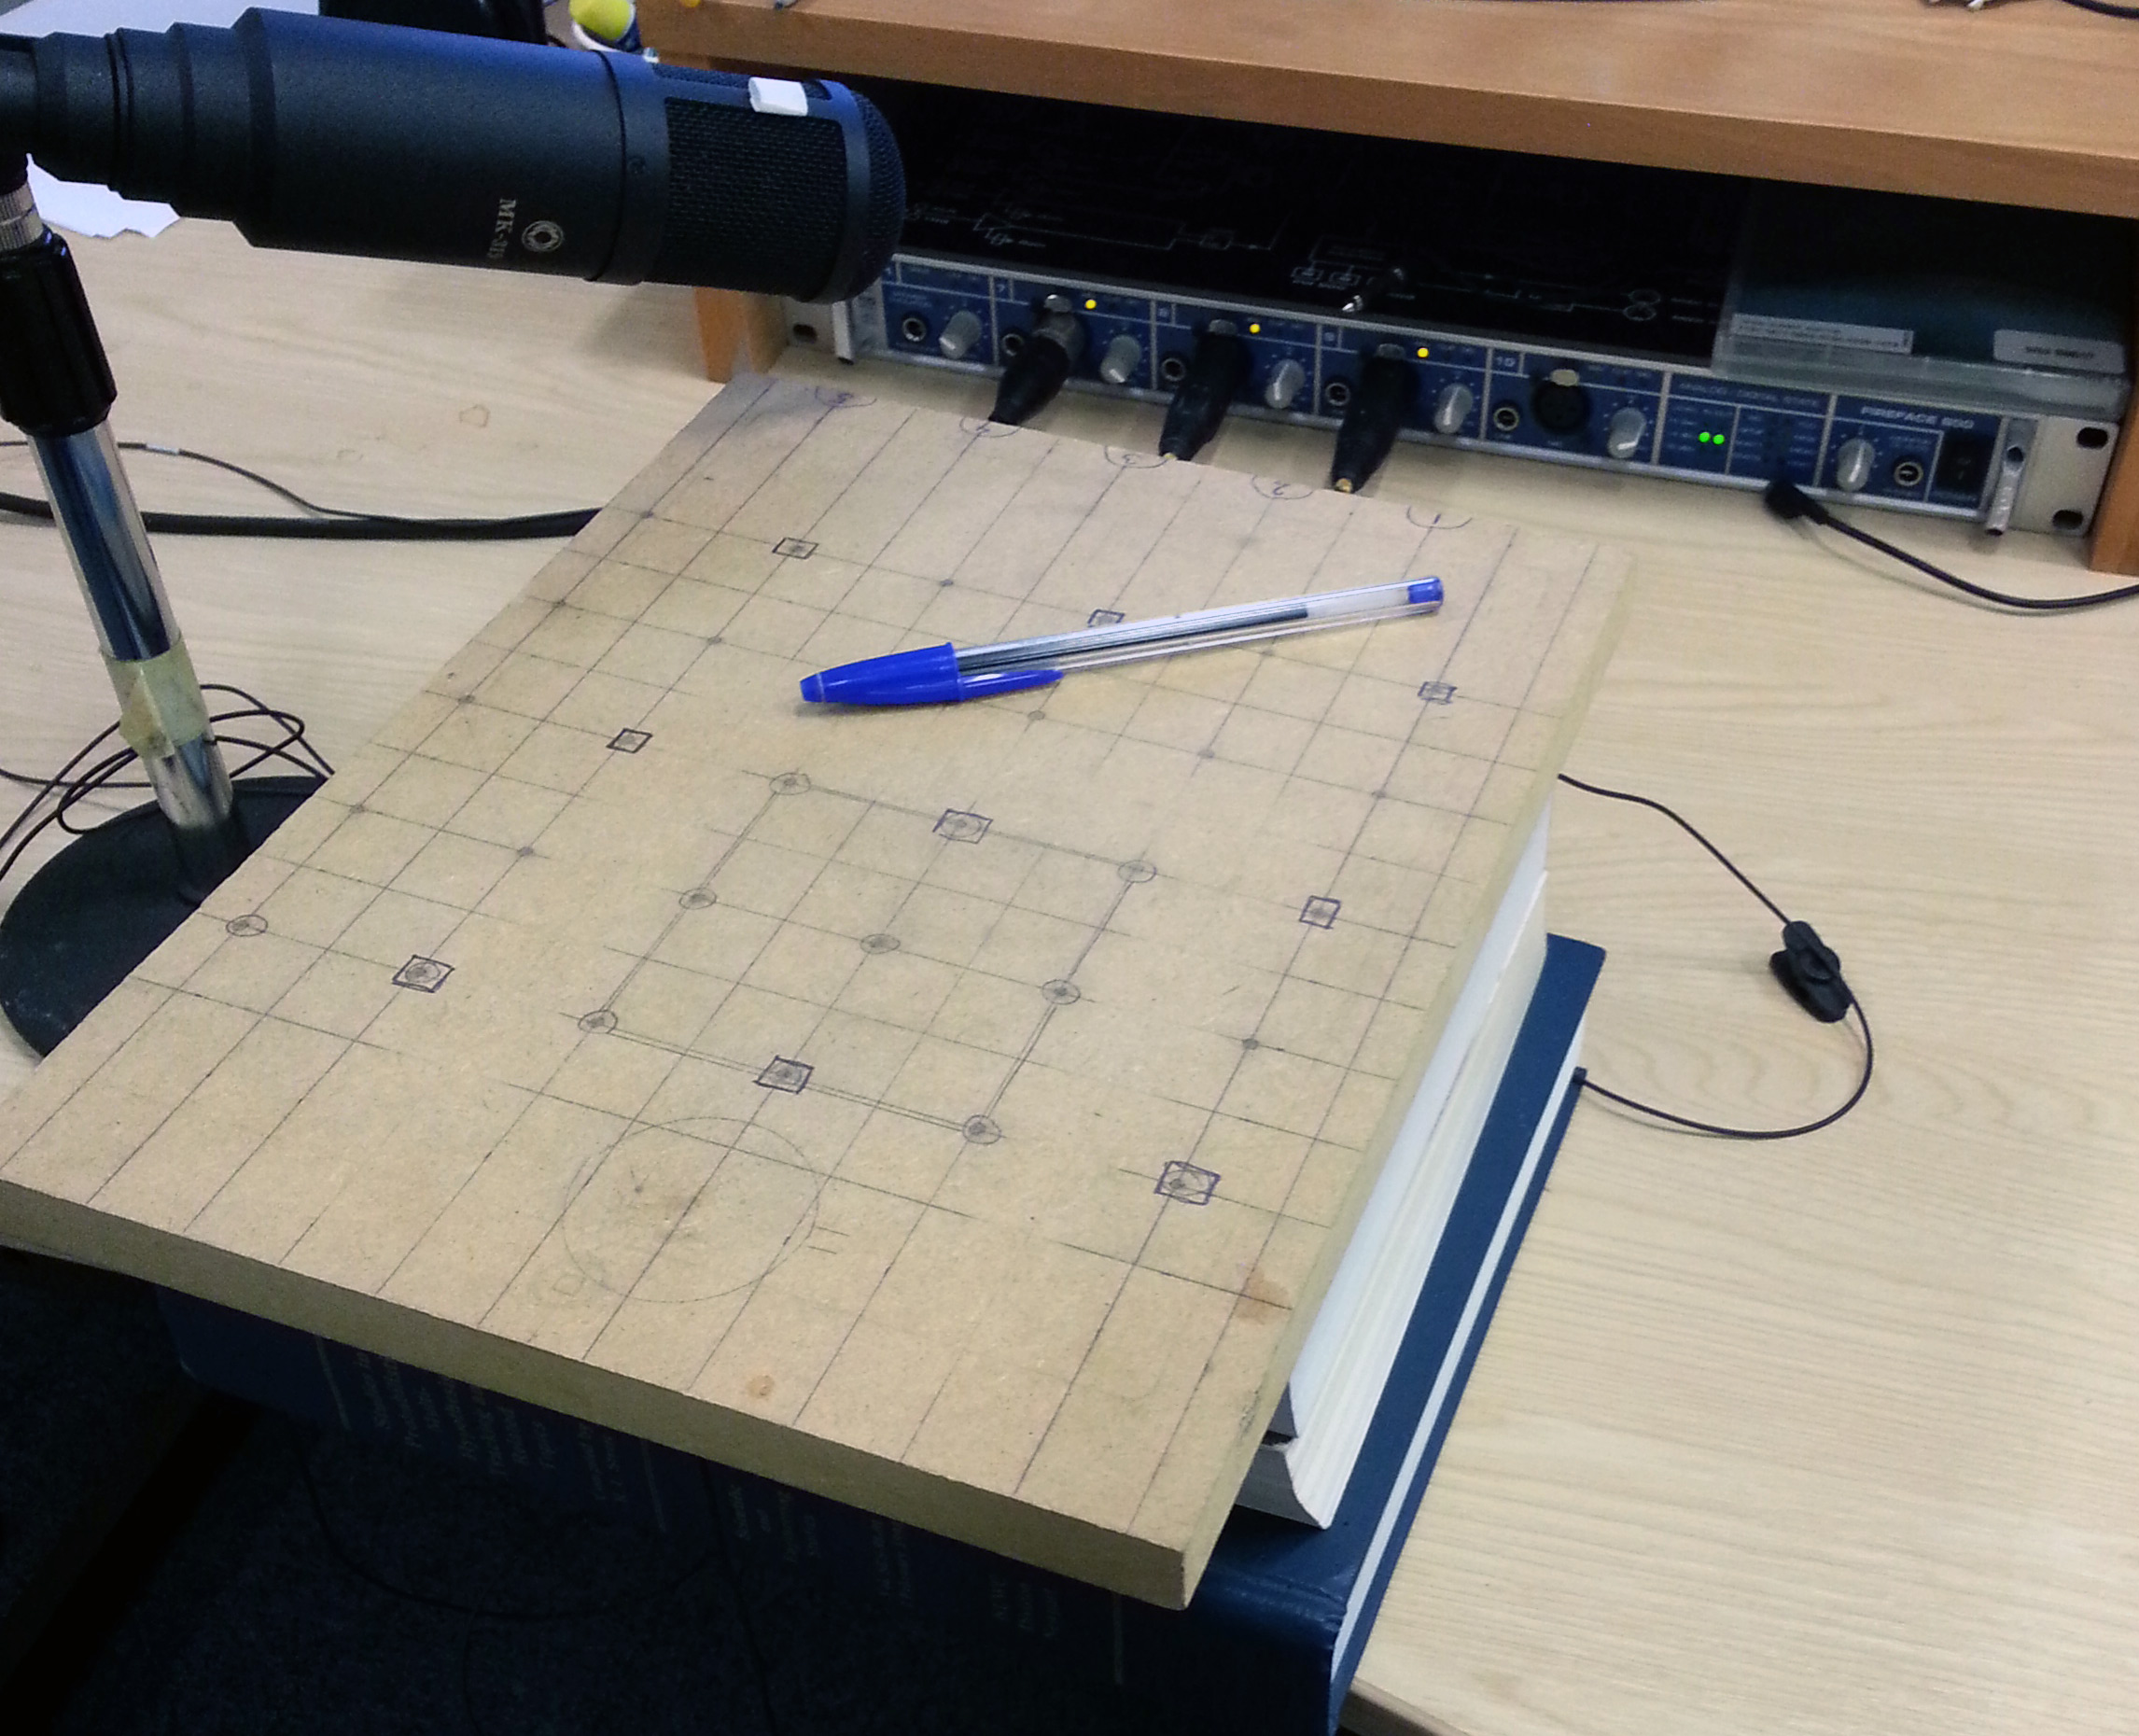
\includegraphics[width=7cm]{wholesystem}
  \caption{The entire multichannel APR system setup.}
  \label{fig:sub1}
\end{subfigure}%
\begin{subfigure}{.5\textwidth}
  \centering
  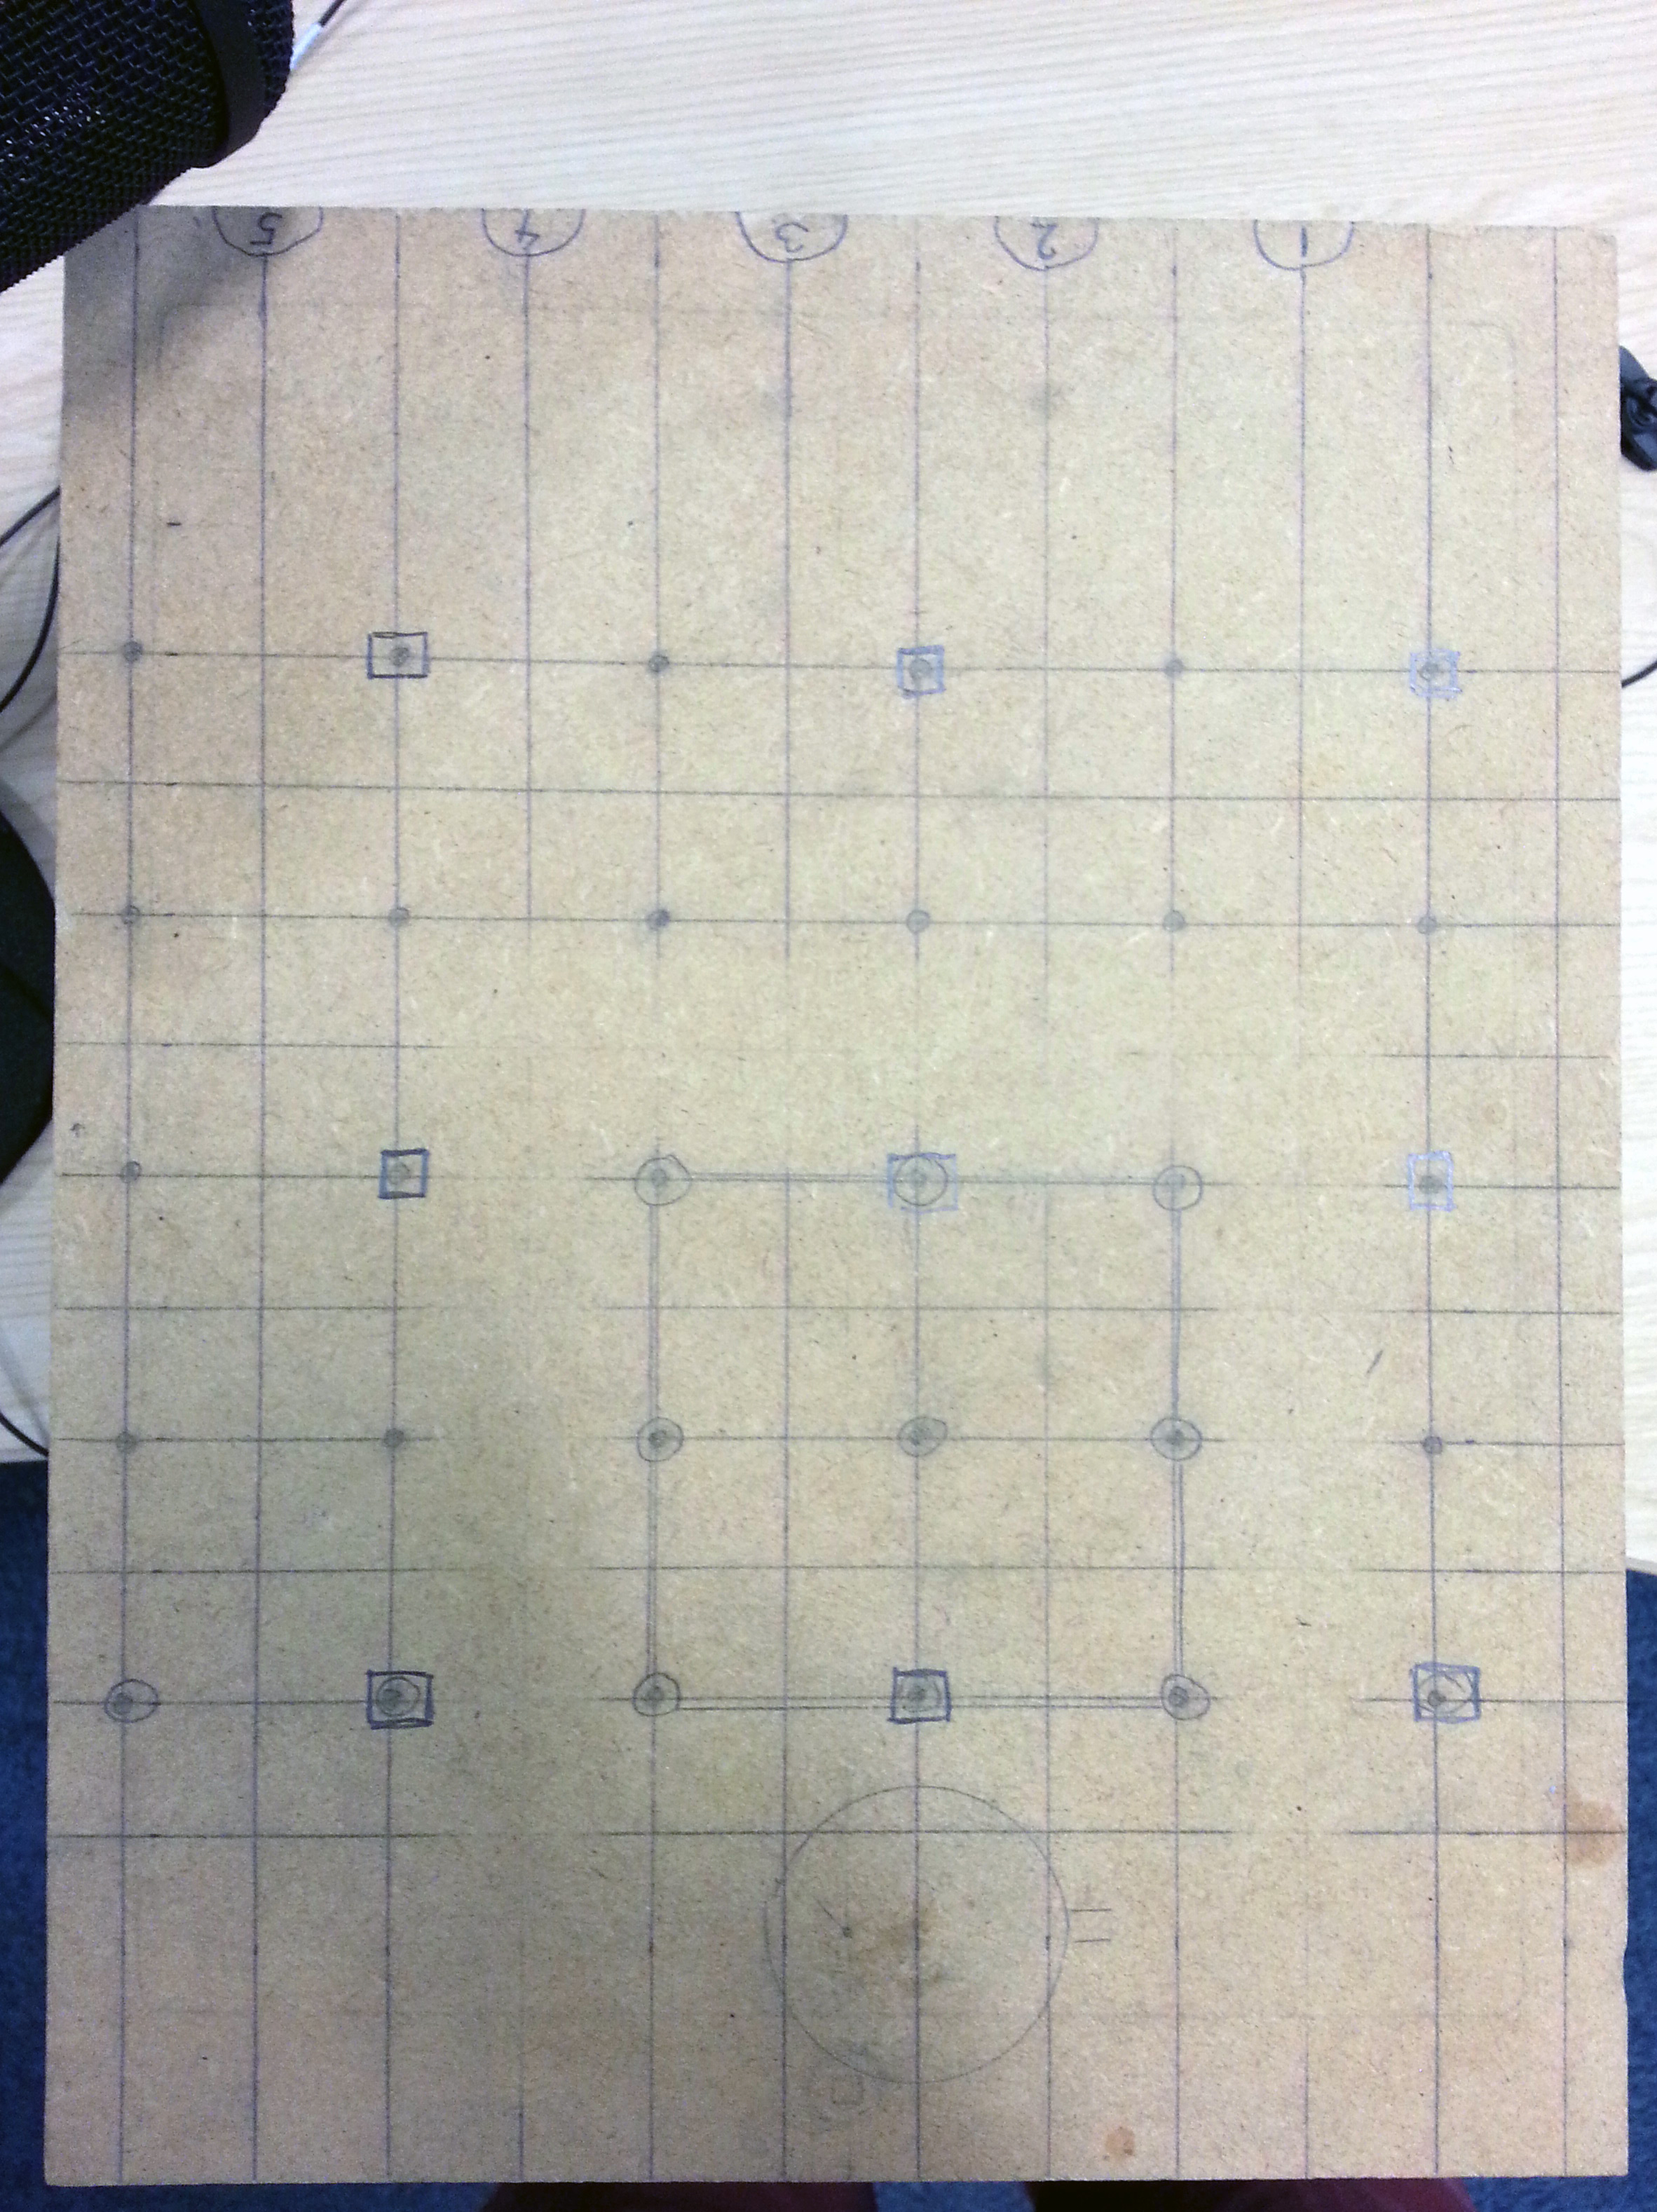
\includegraphics[width=6cm]{surface}
  \caption{The front face of the surface.}
  \label{fig:sub2}
\end{subfigure}
\caption{The multichannel system setup}
\label{fig:multiAPRsystemwhole}
\end{figure}

Microphone 1, seen in Figures~\ref{fig:mic1}(a) and (b), was an Oktava MK-319 large diaphragm condenser microphone. This microphone was positioned slightly above and outside the edge of the surface. Figure~\ref{fig:mic23}(a) and (b) shows microphones 2 and 3, respectively. These were DPA 4060 miniature condenser microphones. All microphones were omnidirectional with no padding or equalizing applied. As noted in Figure~\ref{fig:mic23}(a) and (b) microphones 2 and 3 were positioned into the drilled holes in the back of the surface and held in place with low density foam.

\begin{figure}
\begin{minipage}[b]{1.0\linewidth}
  \centering
  \centerline{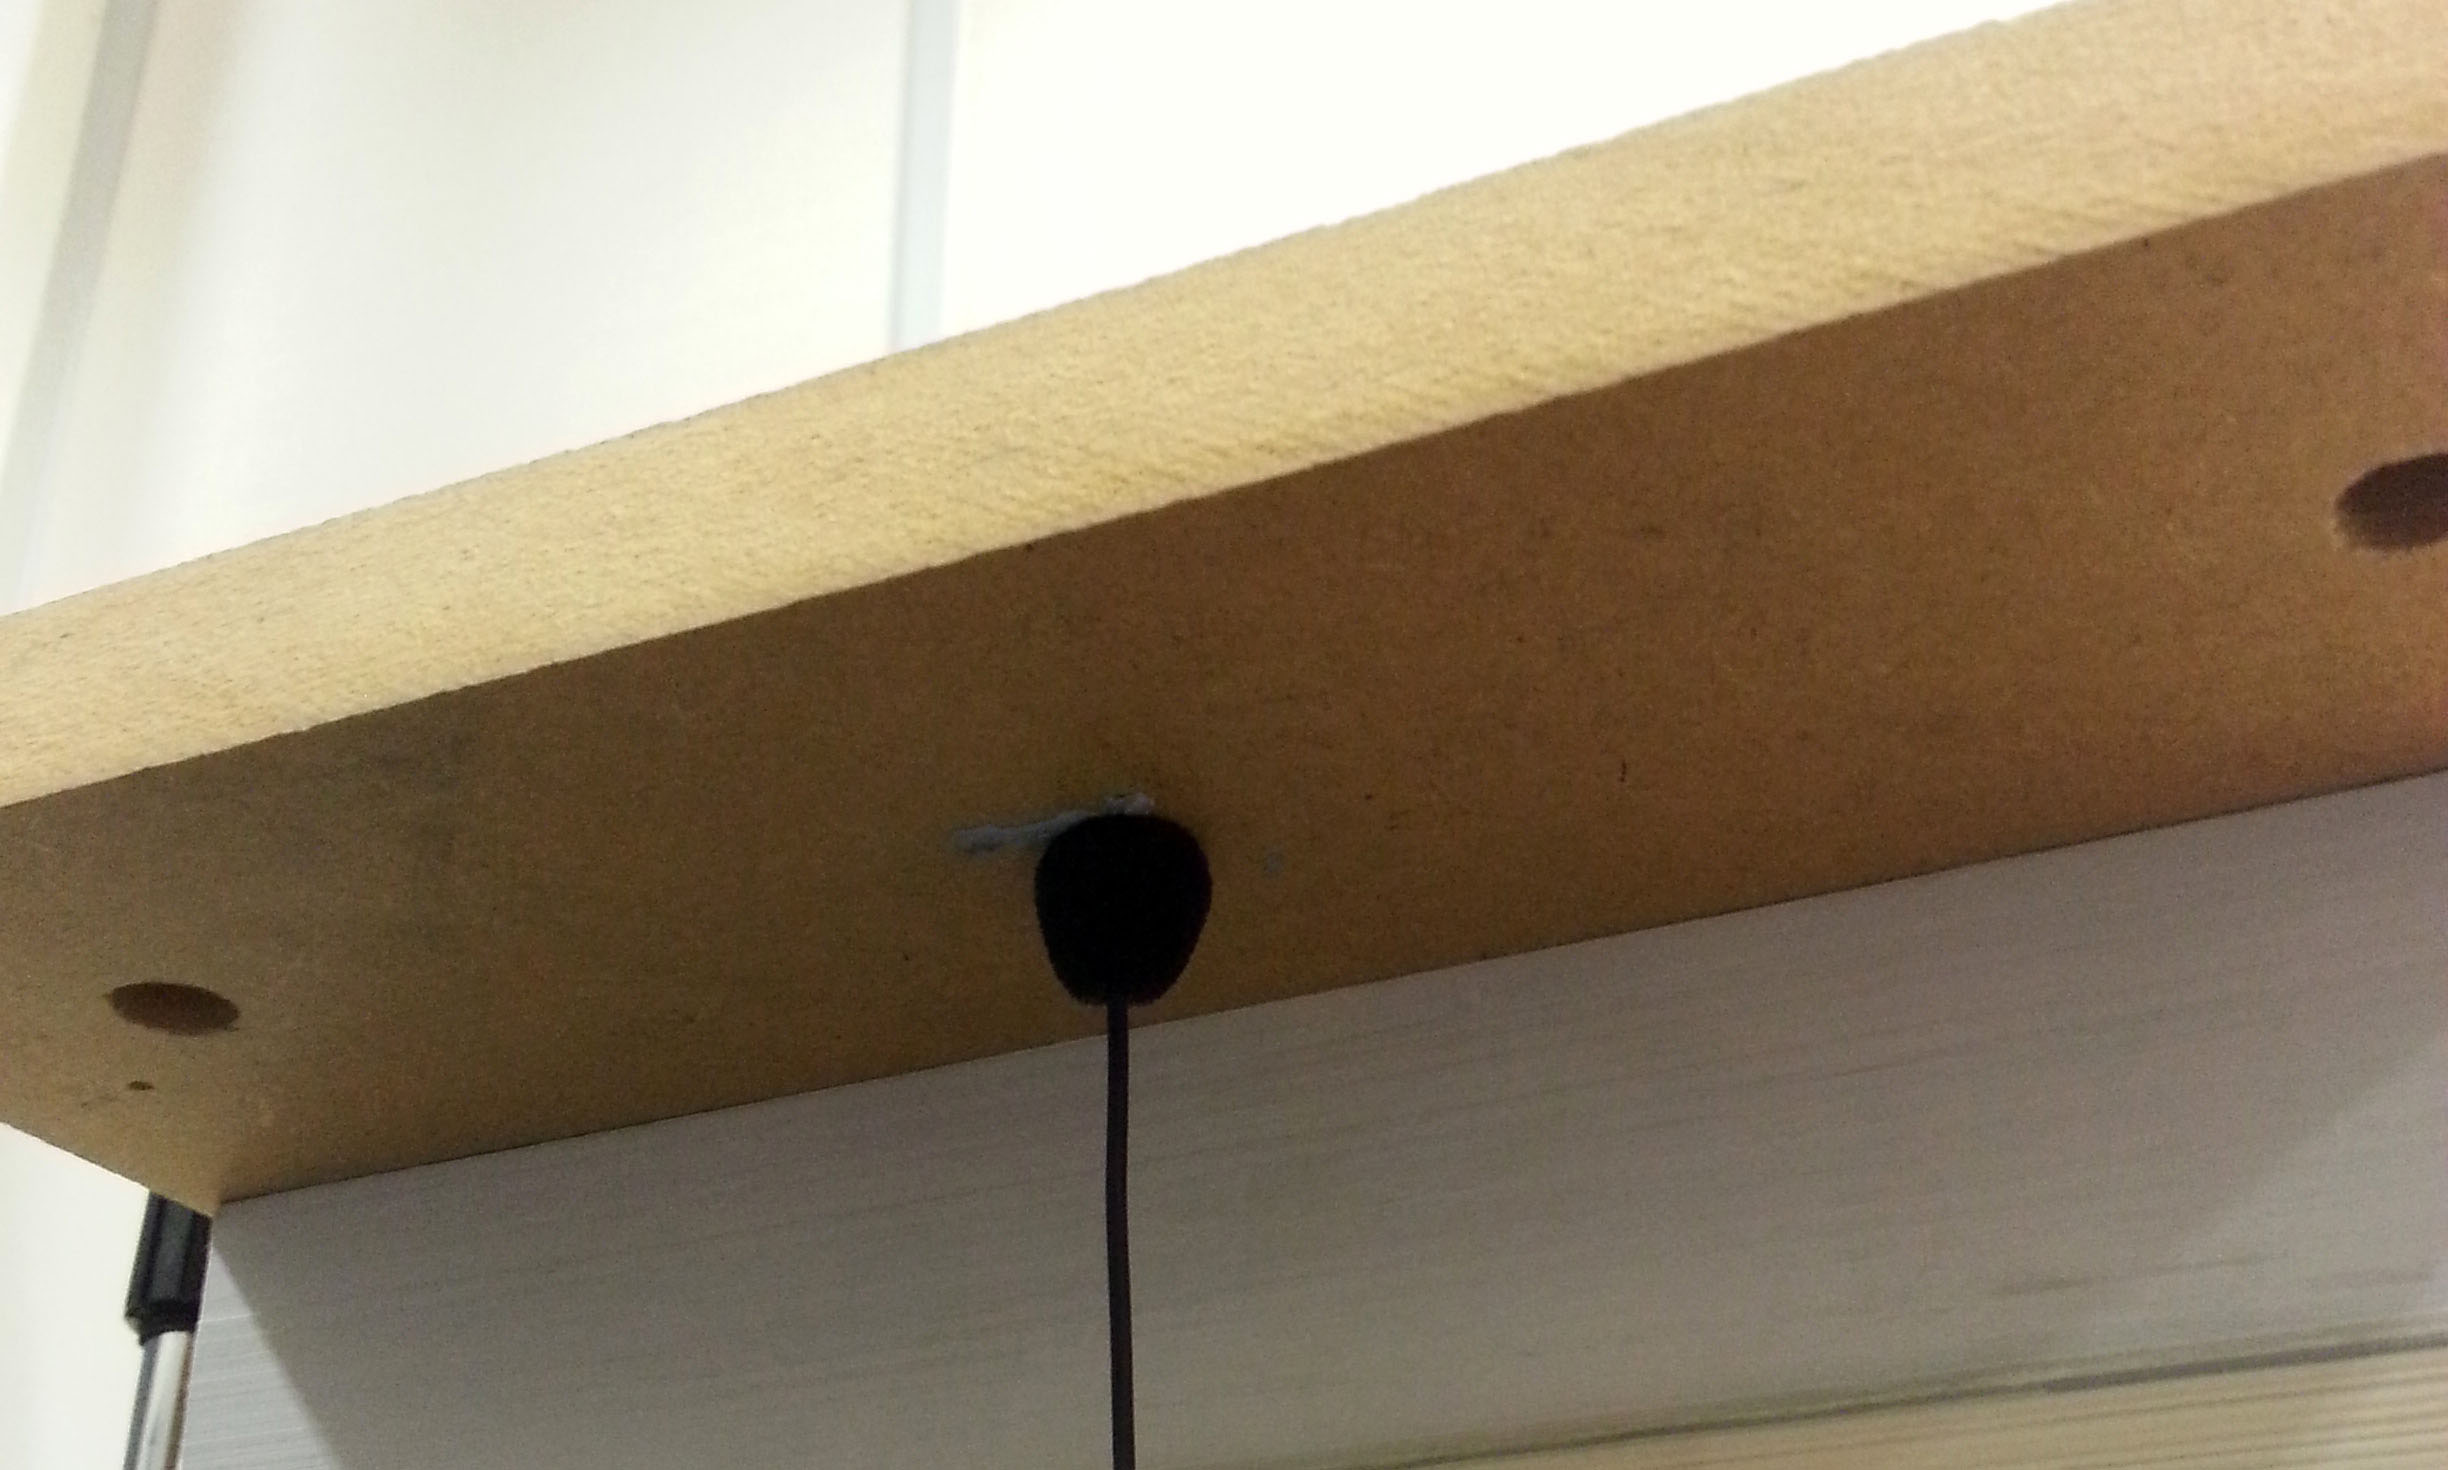
\includegraphics[width=10cm]{mic2}}
  %\vspace{.5cm}
  \centerline{(a) Microphone 2}\medskip
\end{minipage}
\begin{minipage}[b]{1.0\linewidth}
  \centering
  \centerline{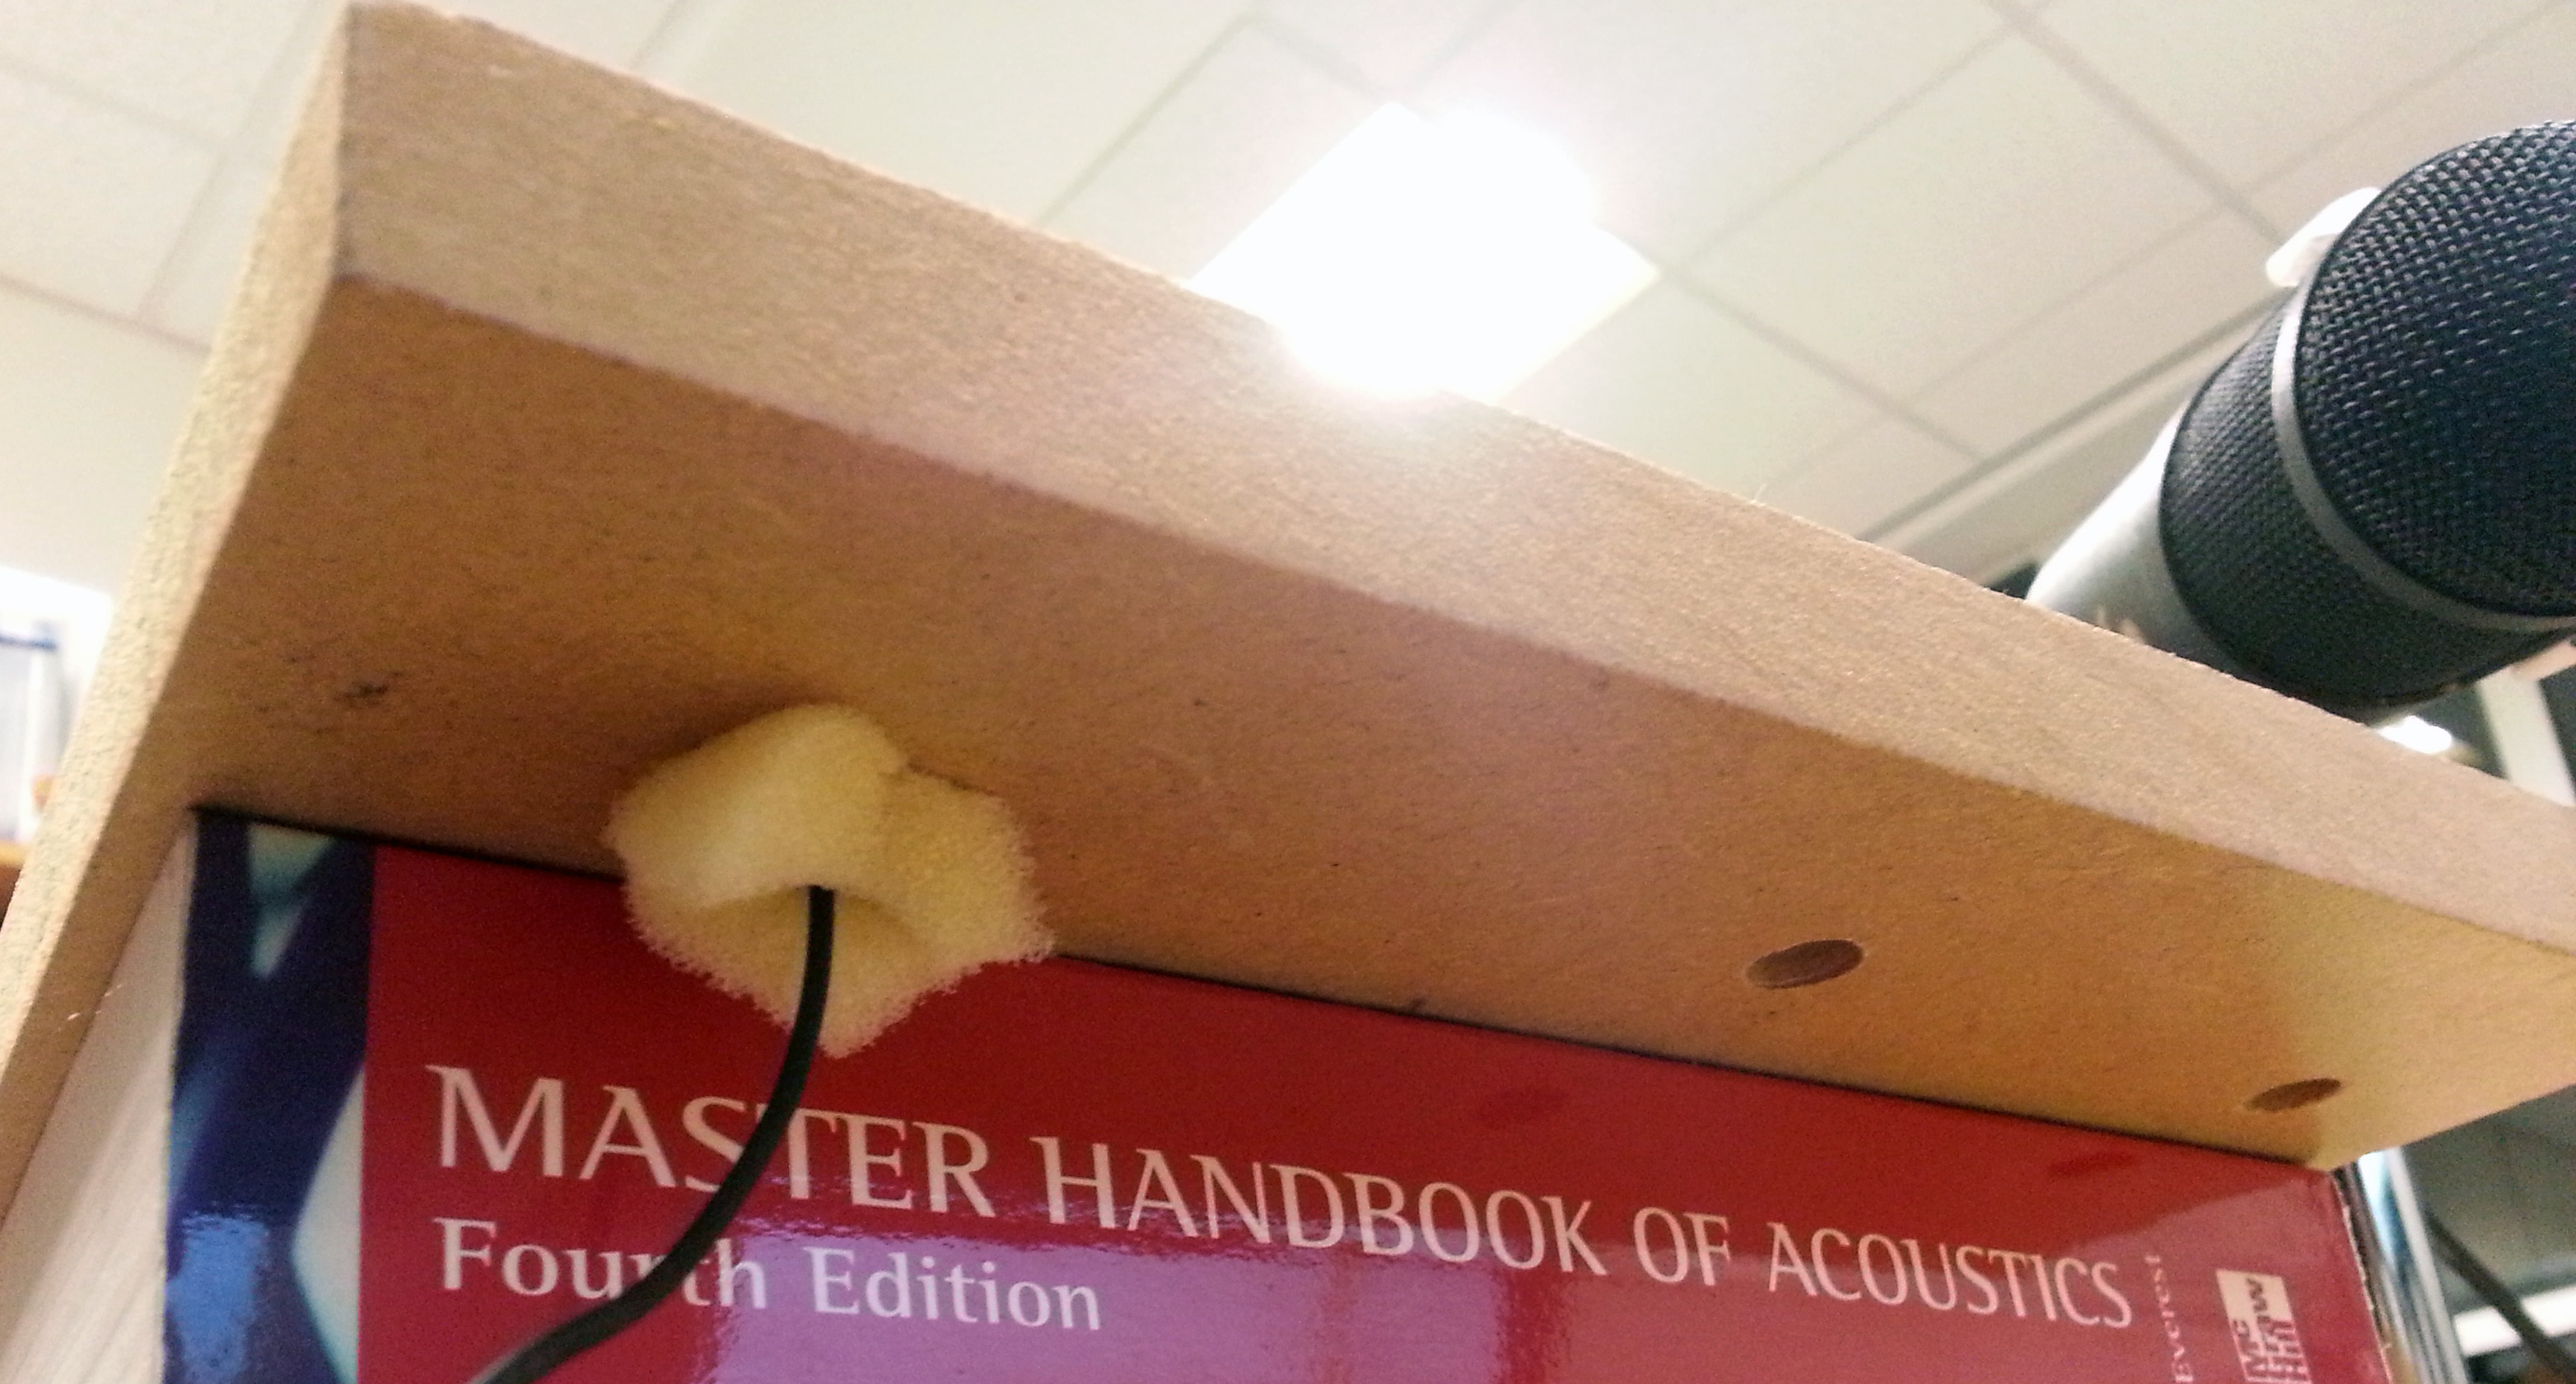
\includegraphics[width=10cm]{mic3}}
  %\begin{picture}(0,0)
%\put(-120,382){(a)}
%\put(-120,195){(b)}
%\end{picture}
 %\vspace{1.5cm}
  \centerline{(b) Microphone 3}\medskip
\end{minipage}
\caption{Microphones 2 and 3 embedded in the back of the surface.}
\label{fig:mic23}
\end{figure}


\begin{figure}
\centering
\begin{subfigure}{.5\textwidth}
  \centering
  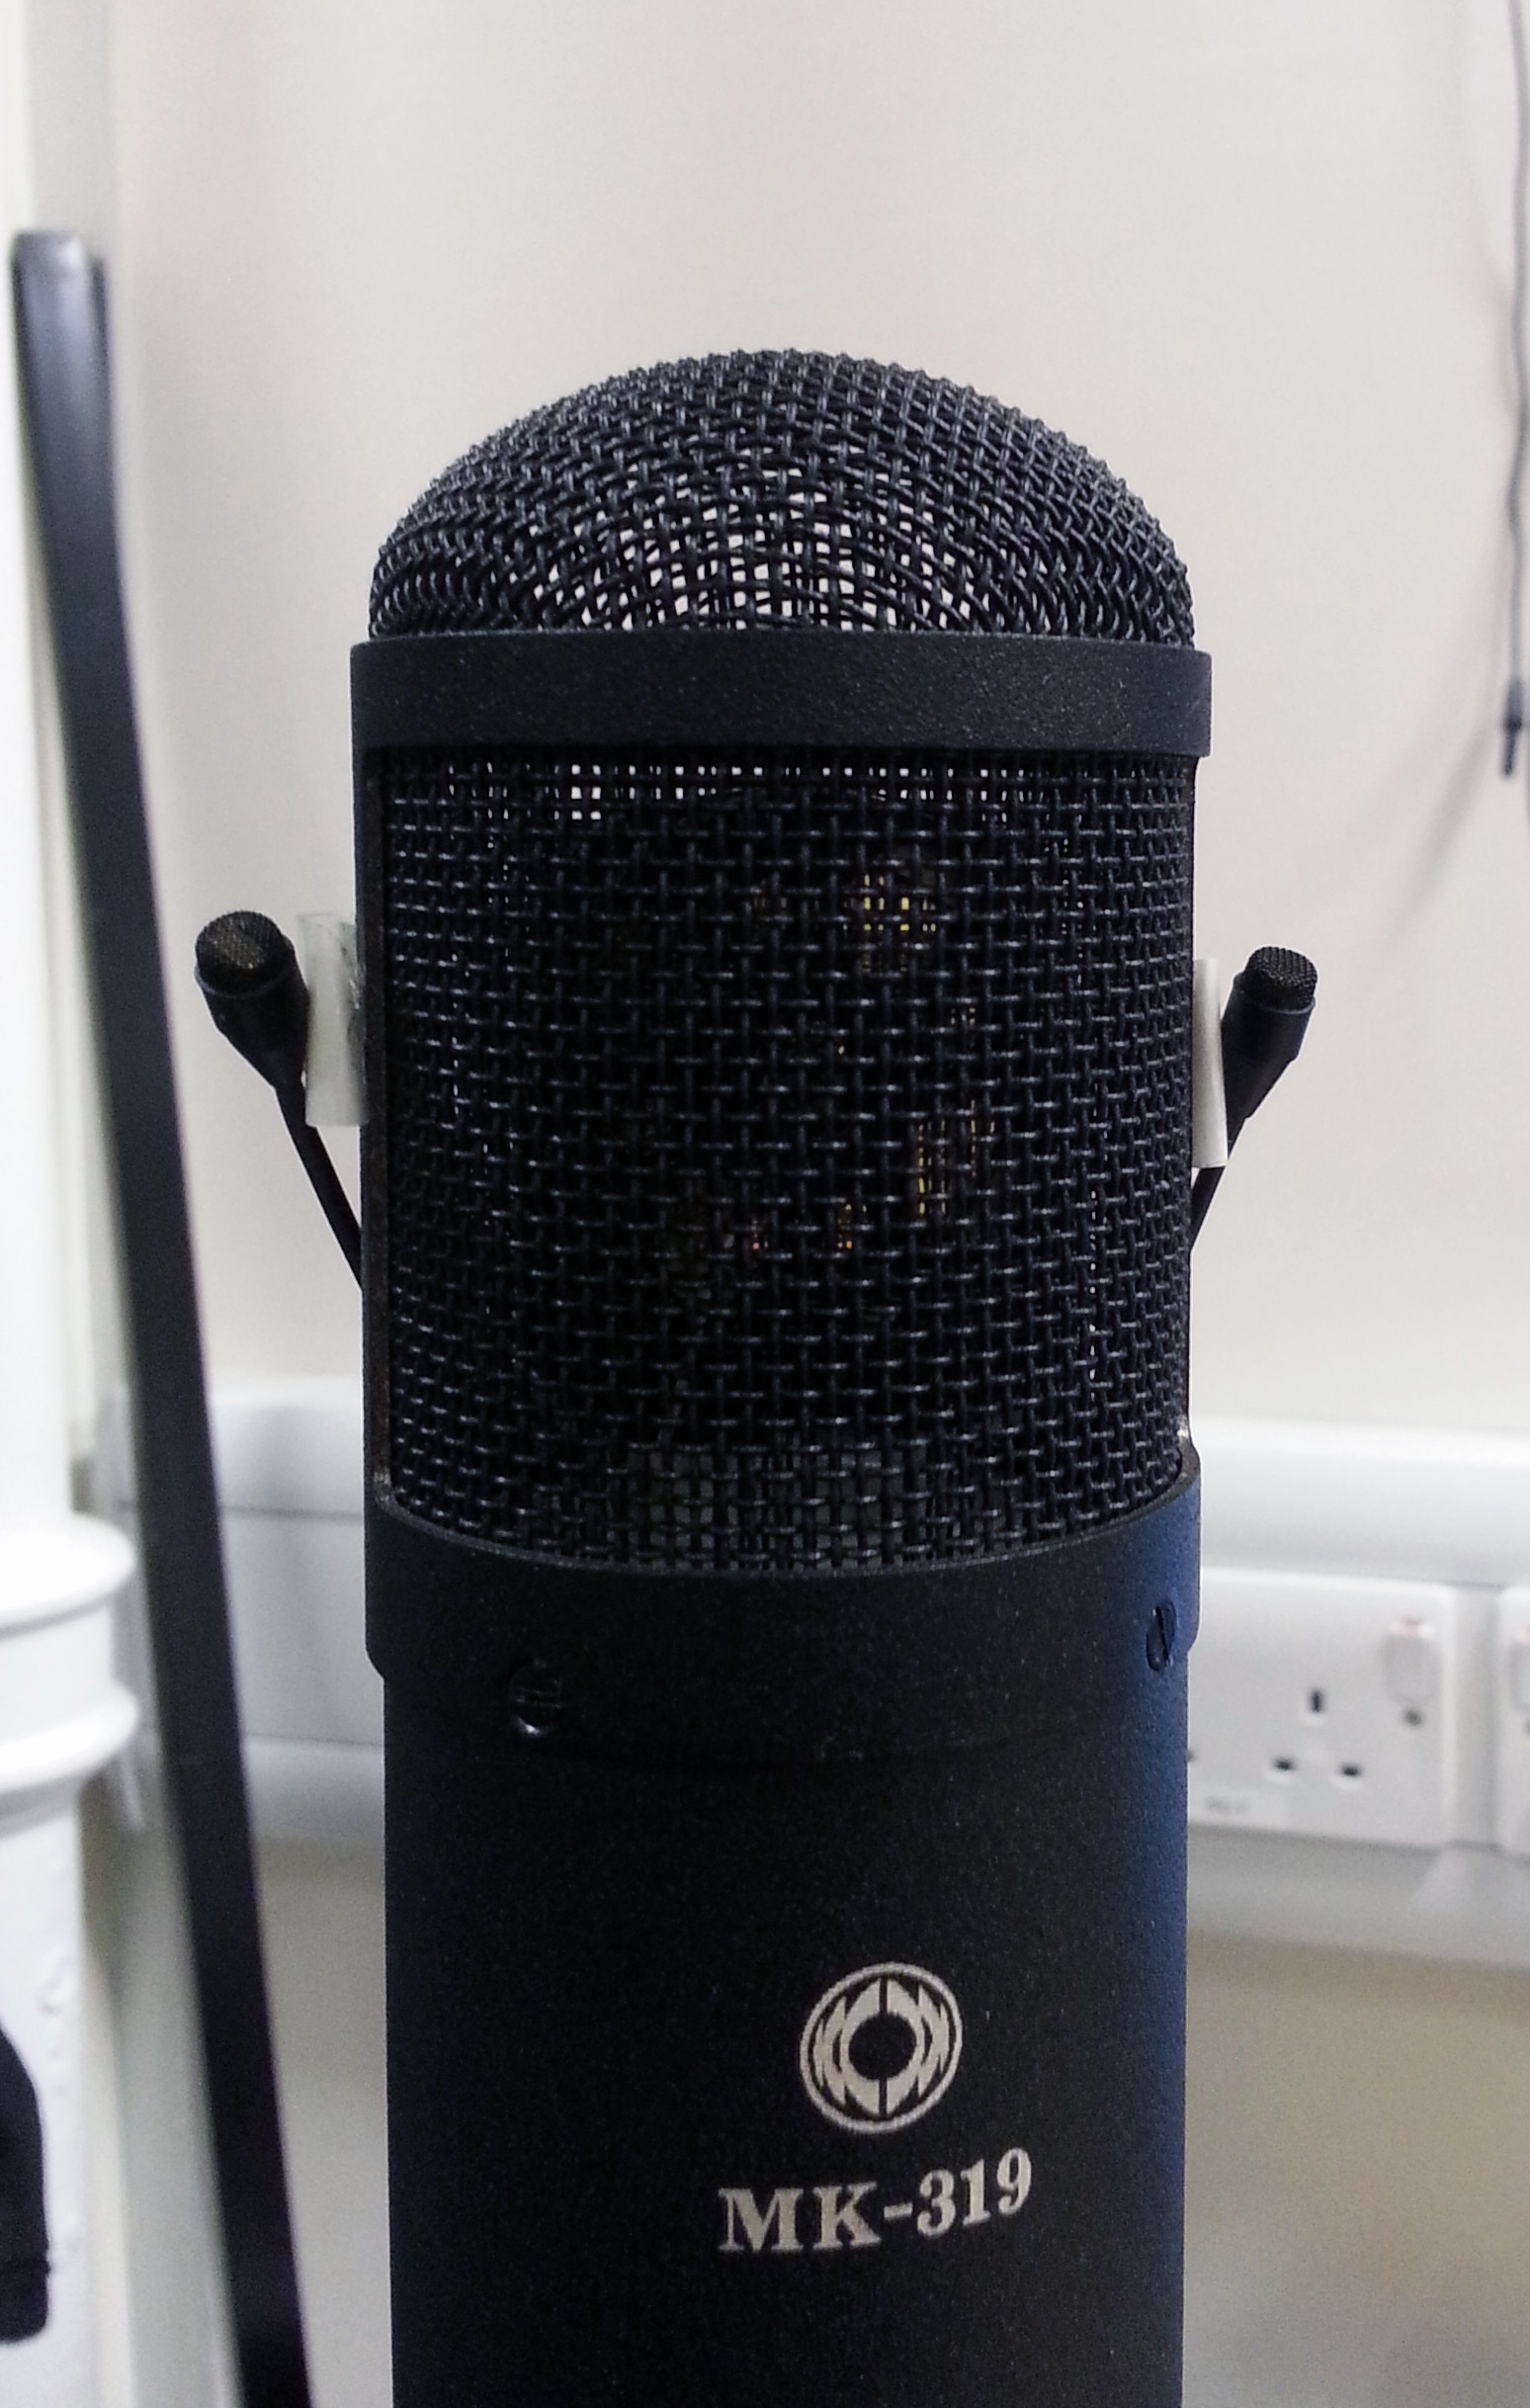
\includegraphics[width=5cm]{micsAlign}
  \caption{A subfigure}
  \label{fig:sub1}
\end{subfigure}%
\begin{subfigure}{.5\textwidth}
  \centering
  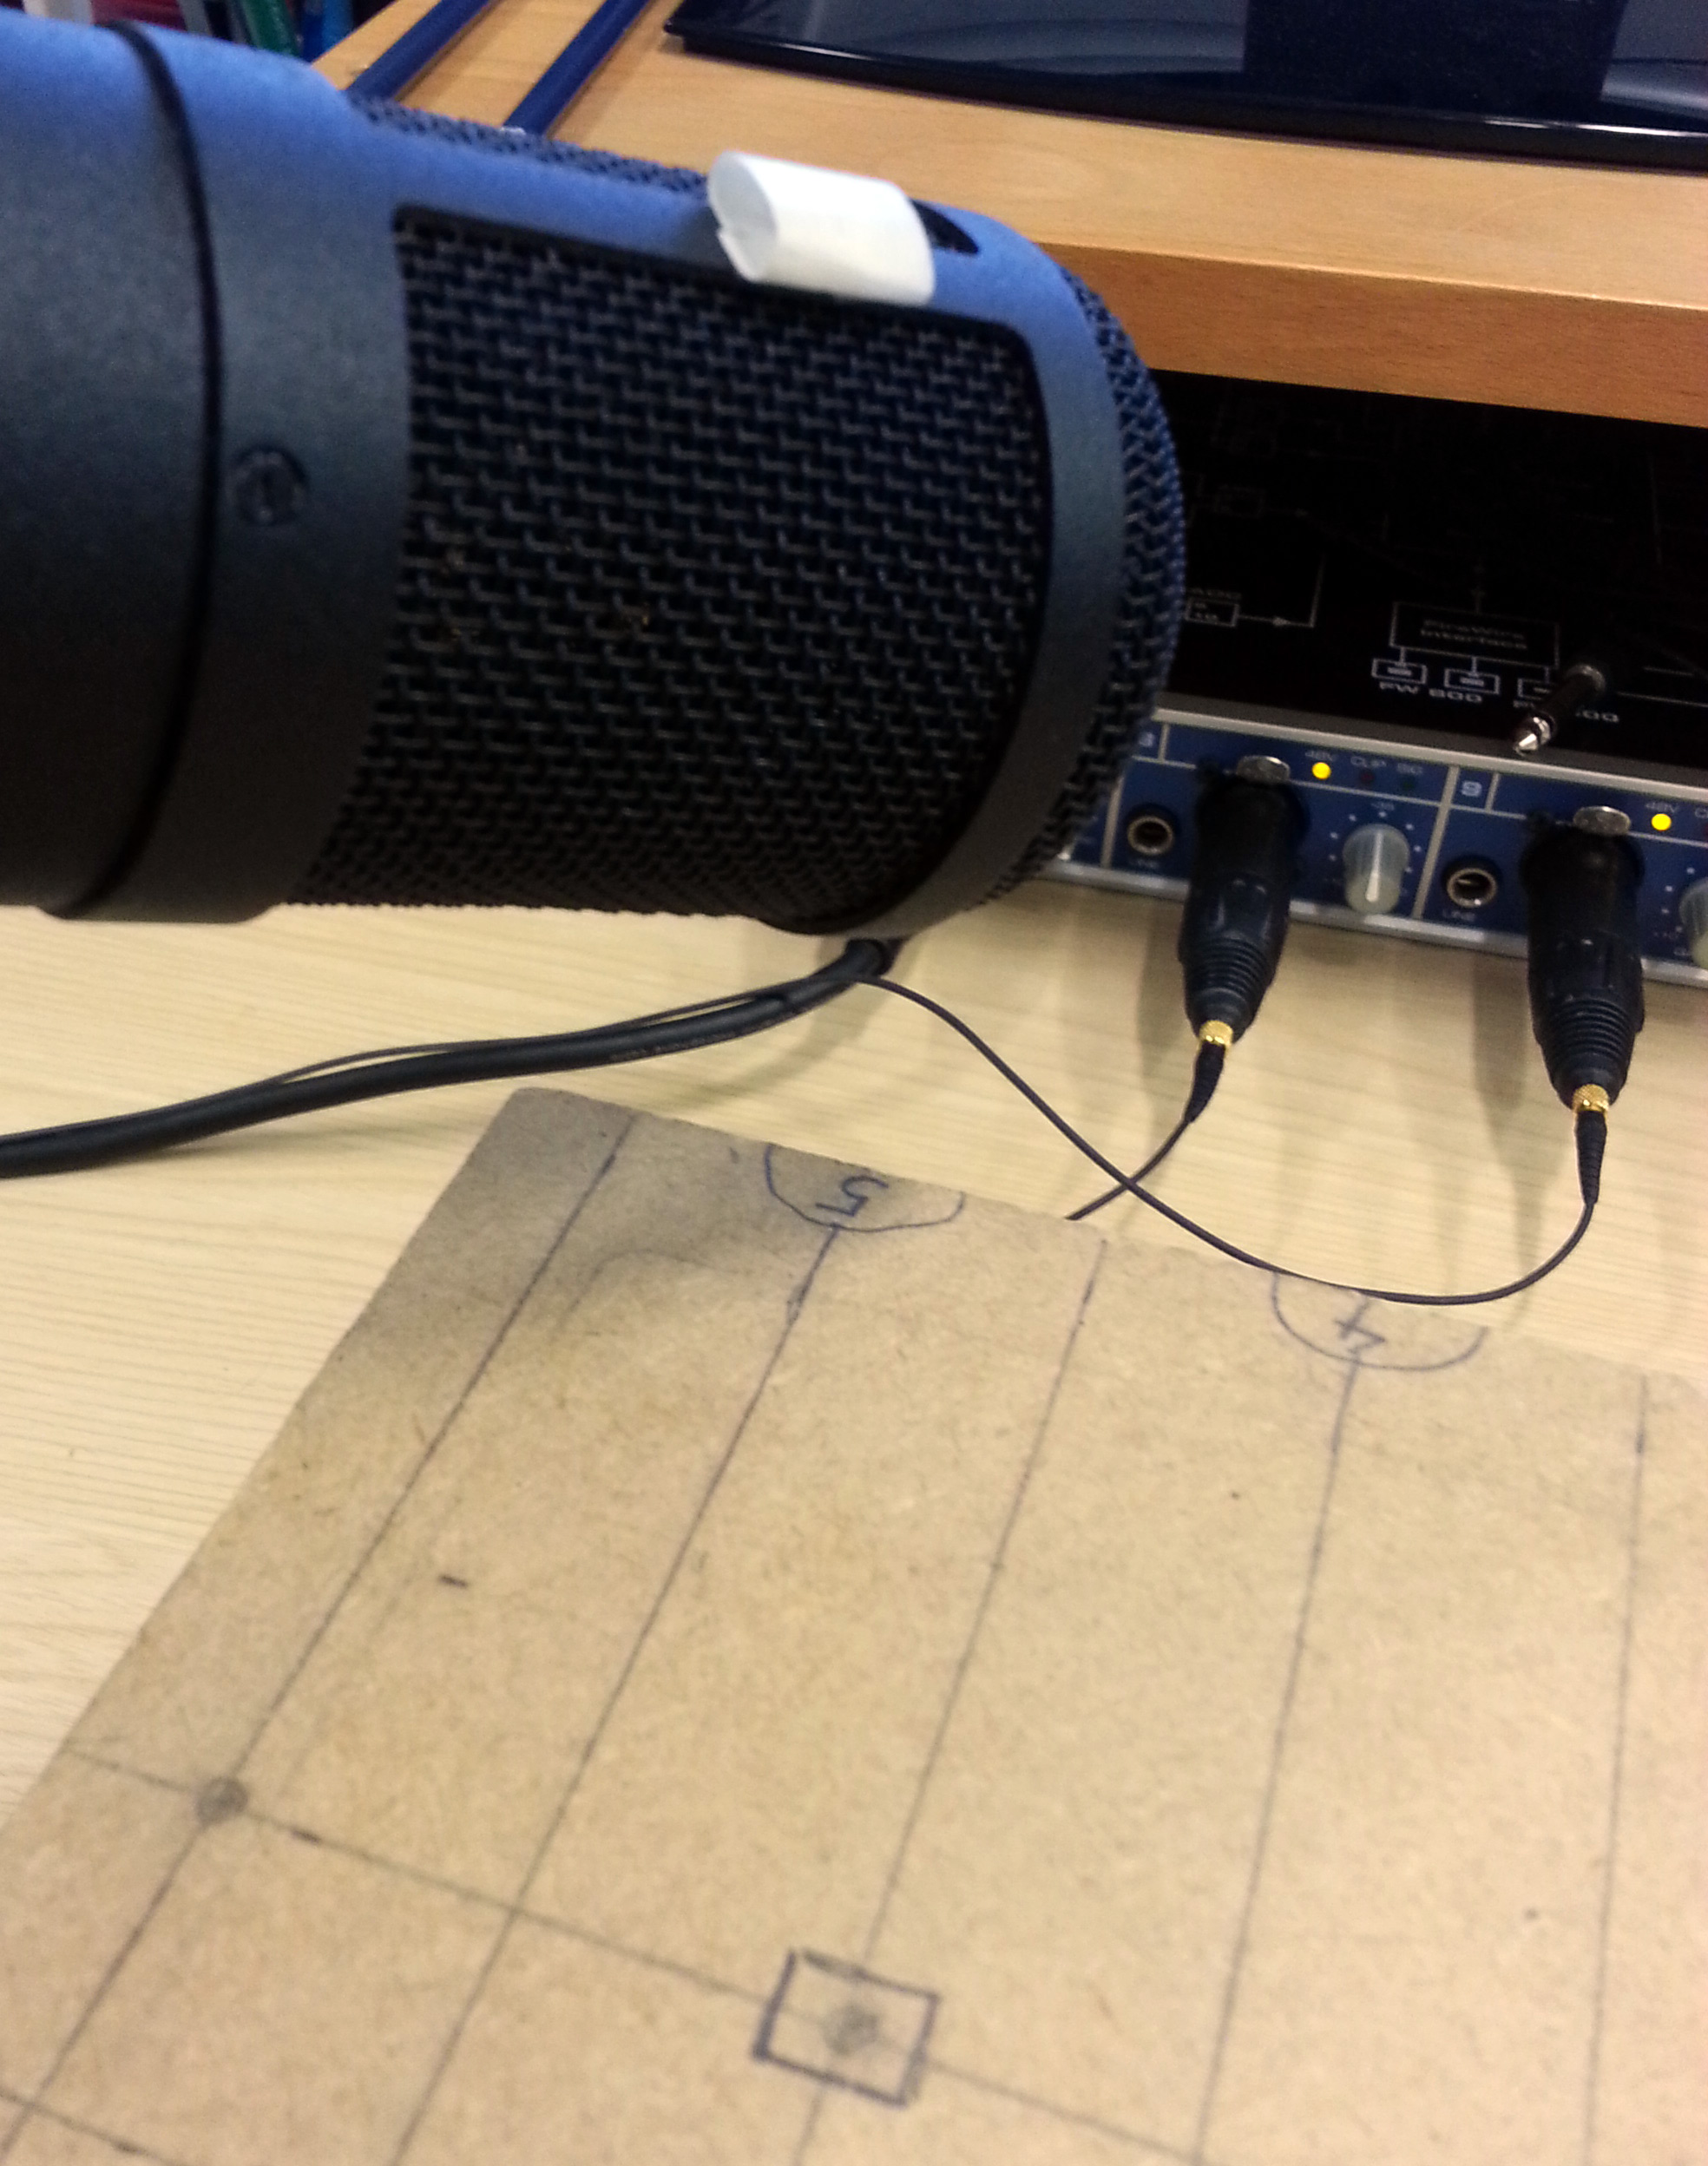
\includegraphics[width=6cm]{mic1}
  \caption{A subfigure}
  \label{fig:sub2}
\end{subfigure}
\caption{A figure with two subfigures}
\label{fig:mic1}
\end{figure}

The AD converters used was an RME Firface 800 and can be seen in Figure~\ref{fig:multiAPRsystemwhole}(a). All data was sampled at 48 kHz at 16 bit.

% ------------------------------------------------------------------------

%%% Local Variables:
%%% mode: latex
%%% TeX-master: "../thesis"
%%% End:
